\documentclass[tikz,border=12pt]{standalone}
% Estilo comum dos esquemas vetoriais das aulas da GA033.
\usepackage[T1]{fontenc}
\usepackage[utf8]{inputenc}
\usepackage{lmodern}
\usepackage{amsmath,amssymb}
\usetikzlibrary{arrows.meta,positioning,calc,fit,matrix,decorations.pathreplacing,backgrounds,shapes.geometric}
\definecolor{lnccblue}{HTML}{075AC0}
\definecolor{ink}{HTML}{242A31}
\definecolor{muted}{HTML}{647080}
\definecolor{lightblue}{HTML}{EFF5FC}
\definecolor{teal}{HTML}{197C83}
\definecolor{orange}{HTML}{BC6A16}
\tikzset{
  every node/.style={font=\sffamily\fontsize{15}{18}\selectfont,text=ink},
  box/.style={draw=lnccblue,line width=0.9pt,fill=lightblue,inner sep=9pt,align=center},
  flow/.style={-{Stealth[length=3mm,width=2mm]},draw=lnccblue,line width=1pt},
  point/.style={circle,draw=lnccblue,fill=white,line width=1.2pt,minimum size=3.2mm,inner sep=0pt},
  label/.style={font=\sffamily\fontsize{13}{16}\selectfont,text=muted},
  heading/.style={font=\sffamily\bfseries\fontsize{16}{19}\selectfont,text=lnccblue}
}
% Impede setas horizontais involuntariamente invertidas após editar os nós.
\newdimen\origemseta
\newdimen\destinoseta
\newcommand{\verificarsetadireita}[2]{%
  \pgfextractx{\origemseta}{\pgfpointanchor{#1}{east}}%
  \pgfextractx{\destinoseta}{\pgfpointanchor{#2}{west}}%
  \advance\origemseta by 4mm%
  \ifdim\destinoseta>\origemseta\else
    \PackageError{diagramas}{Conector sem espaco entre #1 e #2}{Afaste os nos antes de compilar.}%
  \fi
}

\begin{document}
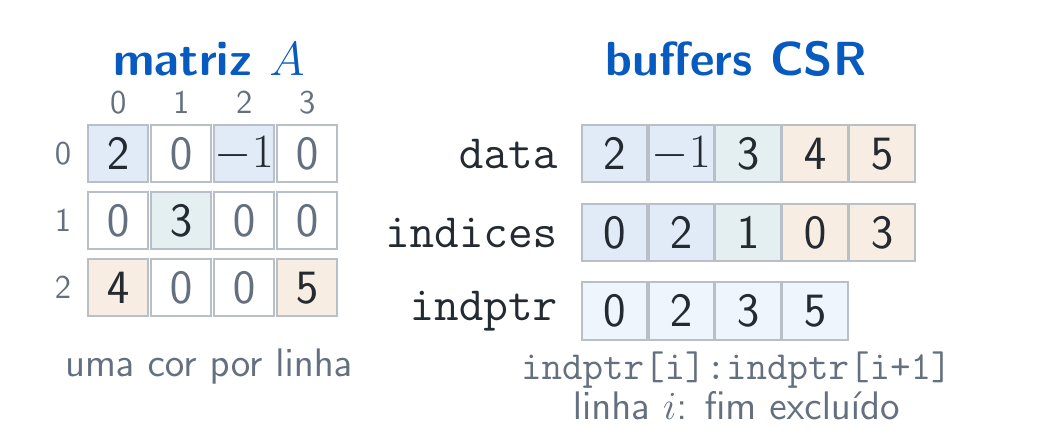
\begin{tikzpicture}[x=1cm,y=1cm,
  every node/.append style={font=\sffamily\fontsize{16}{19}\selectfont},
  dense/.style={draw=muted!45,line width=.7pt,minimum width=.76cm,minimum height=.73cm,inner sep=0pt},
  entry/.style={draw=muted!45,line width=.7pt,minimum width=.83cm,minimum height=.73cm,inner sep=0pt}]
  \path[use as bounding box] (0,0) rectangle (12.8,4.9);
  \node[heading] at (2.3,4.5) {matriz $A$};
  \node[heading] at (9.0,4.5) {buffers CSR};
  \foreach \j in {0,1,2,3} {
    \node[text=muted,font=\sffamily\fontsize{13}{16}\selectfont] at ({1.15+.8*\j},3.95) {\j};
  }
  \foreach \i in {0,1,2} {
    \node[text=muted,font=\sffamily\fontsize{13}{16}\selectfont] at (.45,{3.3-.85*\i}) {\i};
  }
  \node[dense,fill=lnccblue!12] at (1.15,3.3) {2};
  \node[dense,text=muted] at (1.95,3.3) {0};
  \node[dense,fill=lnccblue!12] at (2.75,3.3) {$-1$};
  \node[dense,text=muted] at (3.55,3.3) {0};
  \node[dense,text=muted] at (1.15,2.45) {0};
  \node[dense,fill=teal!12] at (1.95,2.45) {3};
  \node[dense,text=muted] at (2.75,2.45) {0};
  \node[dense,text=muted] at (3.55,2.45) {0};
  \node[dense,fill=orange!12] at (1.15,1.6) {4};
  \node[dense,text=muted] at (1.95,1.6) {0};
  \node[dense,text=muted] at (2.75,1.6) {0};
  \node[dense,fill=orange!12] at (3.55,1.6) {5};
  \node[anchor=east] at (6.85,3.3) {\texttt{data}};
  \node[entry,fill=lnccblue!12] at (7.45,3.3) {2};
  \node[entry,fill=lnccblue!12] at (8.3,3.3) {$-1$};
  \node[entry,fill=teal!12] at (9.15,3.3) {3};
  \node[entry,fill=orange!12] at (10.0,3.3) {4};
  \node[entry,fill=orange!12] at (10.85,3.3) {5};
  \node[anchor=east] at (6.85,2.3) {\texttt{indices}};
  \node[entry,fill=lnccblue!12] at (7.45,2.3) {0};
  \node[entry,fill=lnccblue!12] at (8.3,2.3) {2};
  \node[entry,fill=teal!12] at (9.15,2.3) {1};
  \node[entry,fill=orange!12] at (10.0,2.3) {0};
  \node[entry,fill=orange!12] at (10.85,2.3) {3};
  \node[anchor=east] at (6.85,1.3) {\texttt{indptr}};
  \node[entry,fill=lightblue] at (7.45,1.3) {0};
  \node[entry,fill=lightblue] at (8.3,1.3) {2};
  \node[entry,fill=lightblue] at (9.15,1.3) {3};
  \node[entry,fill=lightblue] at (10.0,1.3) {5};
  \node[text=muted,font=\sffamily\fontsize{14}{17}\selectfont] at (2.3,.6) {uma cor por linha};
  \node[text=muted,font=\sffamily\fontsize{14}{17}\selectfont] at (9.0,.55) {\texttt{indptr[i]:indptr[i+1]}};
  \node[text=muted,font=\sffamily\fontsize{14}{17}\selectfont] at (9.0,.1) {linha $i$: fim excluído};
\end{tikzpicture}
\end{document}
